\documentclass{standalone}
\usepackage{tikz}
\usepackage{ctex,siunitx}
\usepackage{tkz-euclide}
\usepackage{amsmath}
\usetikzlibrary{patterns, calc}
\usetikzlibrary {decorations.pathmorphing, decorations.pathreplacing, decorations.shapes,}
\begin{document}
\small
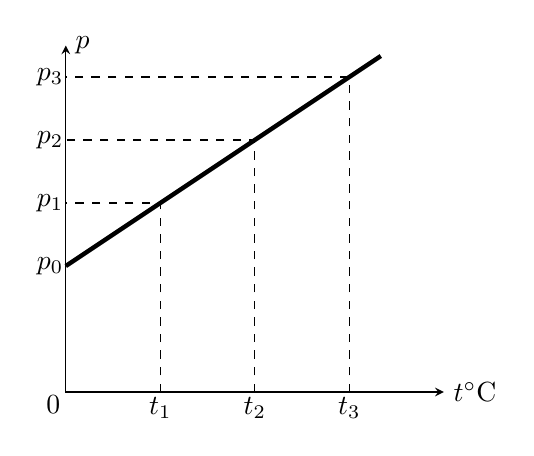
\begin{tikzpicture}[>=stealth,scale=0.8]
  \draw[<->] (0,6.5)node [right]{$p$}--(0,1)--(6,1) node [right]{{$t^\circ$C}};
  \draw[color=black, ultra thick] (0,3)--(5,6+1/3);
  \draw [dashed] (1.5,+1)--(1.5,4)--(0,4);
  \draw [dashed] (3,+1)--(3,5)--(0,5);
  \draw [dashed] (4.5,+1)--(4.5,6)--(0,6);
  \node at (-.2,-.2+1){$0$};
  \node at (1.5,-.25+1){$t_1$};\node at (3,-.25+1){$t_2$};\node at (4.5,-.25+1){$t_3$};
  \node at (-.25,4){$p_1$};\node at (-.25,5){$p_2$};\node at (-.25,6){$p_3$};
  \node at (-.25,3){$p_0$};
\end{tikzpicture}
\end{document}